\pstart [96 r\textsuperscript{o}] Constructio huc \edtext{redit:}{\lemma{redit}\Bfootnote{\textsc{O. v. Guericke, }\cite{00055}a.a.O., S.~123, Iconismus XVII.\protect\rule[0cm]{2cm}{0cm}}}
   \pend          
    \pstart         Globus \textit{A} aere plenus \edtext{magnitudine Recipientis}{\lemma{}\Afootnote{magnitudine Recipientis \textit{ erg.} \textit{ L}}} ex eo exit Tubus \textit{BC} cupreus amplitudine pollicaris  7. ulnarum huic conjunctus in \textit{C} alius \textit{DE} cui certa spiritus vini\protect\index{Sachverzeichnis}{spiritus!vini} quantitas infunditur. Huic in \textit{C} immittitur tubus alius \textit{KL} in eo natans, in aequilibrium\protect\index{Sachverzeichnis}{aequilibrium} cum spiritu vini\protect\index{Sachverzeichnis}{spiritus!vini} redactus per injectos globulos  plumbeos ne ejus ex superficie  emineat. Tubus clauditur  inde extrahitur tantum aeris ex  Tubo \textit{A} \edtext{tempore}{\lemma{\textit{A}}\Afootnote{ \textit{ (1) }\ nocte \textit{ (2) }\ tempore \textit{ L}}} aliqua medio, quo  pruinosae ac frigidae noctes ingruunt, \edtext{eousque extrahens donec  icuncula}{\lemma{ingruunt,}\Afootnote{ \textit{ (1) }\ ita ut hinc icu \textit{ (2) }\ eousque extrahens donec  icuncula \textit{ L}}} circiter ad medium assurgat, tubo \textit{KL} descendente, quia vinum versus \textit{A}  ascendit. (+ Rectius pro primo usu indeterminata sumatur longitudo, unus annus  tibi ostendet ubi locus medius, exhauries  ergo pro lubitu. Calida tempestate descendet frigida ascendet virunculus. +) Est  et aliud Thermometrum\protect\index{Sachverzeichnis}{thermometrum} Gerickii\protect\index{Namensregister}{\textso{Guericke} (Gerickius, Gerick.), Otto v. 1602\textendash 1686} imaguncula vitrea immittatur in Tubum vitreum  2 vel 3. ulnarum longum, ita ut in eo libere  pendeat, ea calida descendet, frigida ascendet,  media medium in tubo locum tenebit, item appende  ad bilancem vitreum recipientem apertum invenias calida tempestate levius, frigida gravius.
    \pend 
                     \begin{center}                   
                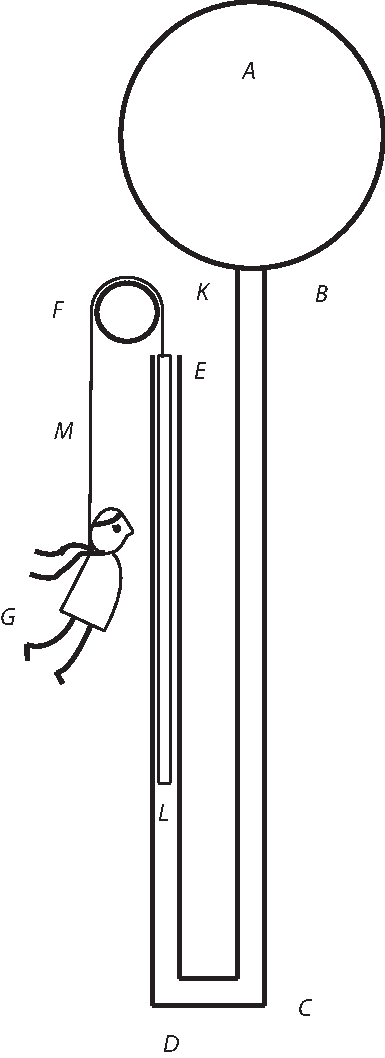
\includegraphics[width=0.27\textwidth]{images/LH35_14_2_96r1}\\\textit{[Fig. 4]} 
                        %\caption{Bildbeschreibung}
                        \end{center}
                        %@ @ @ Dies ist eine Abstandszeile - fuer den Fall, dass mehrere figures hintereinander kommen, ohne dass dazwischen laengerer Text steht. Dies kann zu einer Fahlermeldung fuehren. @ @ @ \\
\pstart 
\textso{Gerick. lib. 4. c. 1.} \edtext{}{\lemma{\textso{1.}}\Bfootnote{\textsc{O. v. Guericke}, \cite{00055}a.a.O., S.~125.}} Virtutes mundanae sunt viventes,  imo animae sentientis. Virtus est aut corporeum  aut incorporeum effluvium. Olfactus est organon excipiendi virtutes corporeas seu odores, ex quibus et aer est. Virtutes incorporeae propagantur etiam per solida,\rule[-1.5cm]{0cm}{0cm}  omnes hoc habent ut in longiore distantia vis  attenuetur ac denique evanescat. Reflectuntur  etiam, ac in subjectis habilibus velut figuntur.
\pend 
\pstart 
\textso{Cap. 2.}\edtext{}{\lemma{\textso{2.}}\Bfootnote{\textsc{O. v. Guericke}, \cite{00055}a.a.O., S.~127f.}} Virtus impulsiva, magis recipitur in corpore magis denso compactove, et majore. \edtext{\textit{Duorum corporum ejusdem materiae et  aeque solidorum, id quod majus est citius}}{\lemma{majore.}\Afootnote{ \textit{ (1) }\ \textit{Accelerationem}\protect\index{Sachverzeichnis}{acceleratio|textit} \textit{ (2) }\ \textit{Duorum [...] citius} \textit{ L}}}\textit{ descendit.}  (+ Ego dubito. +) \textit{Globus plumbeus duarum unciarum  citius multo terram attingit quam unius unciae.}  (+ Dubito. +) Arcus magnus sagittam justo minorem  non eo projiciet quo majorem. \textit{Globus plumbeus  funi alligatus et in gyrum vibratus vel  circumductus quanto major est tanto celerius, inque  majore, circumferentia potest circumduci.} \textit{Res  parva magnae parum virtutis impulsivae imprimere  potest. Sic malleus incudi non sensibilem imprimit  effectum hujus virtutis, unde solea equorum  ferrea ein Huffeisen super incude hominis  ventri imposita malleo et acuto ferro discuti  seu in frusta comminui potest sine ulla hominis laesione.}
\pend 
\pstart 
\textso{Cap. 3.}\edtext{}{\lemma{\textso{3.}}\Bfootnote{\textsc{O. v. Guericke}, \cite{00055}a.a.O., S.~128\textendash130.}} \textit{Virtus impulsiva in  omnem partem operari potest, ut in }\textit{Hollandia}\protect\index{Ortsregister}{Holland (Hollandia)}\textit{ experiuntur  illi, qui super glaciem soleis ferreis induti uno impetu  tam rectum quam circularem cursum instituere  possunt.} (+ Quaerendum quomodo.~+) \textit{Experimentum circa }\textit{vim impulsivam}\protect\index{Sachverzeichnis}{vis!impulsiva}\textit{ circularem. Sit  globus plumbeus }\textit{a}\textit{ mediante filo }\textit{ab}\textit{ alligatus  baculo }\textit{bc}\textit{; hic globulus }\textit{a}\textit{ beneficio istius baculi ab aliquo (si  filum est in debita longitudine vel proportionata distantia), optime in gyrum circumduci vel vibrari potest. Quando autem distantia seu filum nimis longum, contra globulus ad talem distantiam non satis ponderis  habet, circumductio aut perficitur difficillime, aut  denique in nullum volatum seu vibrationem perduci potest.} (+~Videtur ergo tum demum fieri circulatio,  quando impressio satis fortis. An non recepti virtus  subjecti vi impressa\protect\index{Sachverzeichnis}{vis!impressa} pensari potest? Seu an ictus  fortis potest plumae impingi: non videtur,  quia non satis resistit. Hinc experimenta  intuenda, de ultimo termino projectionis ad aliquam distantiam, v. g. arenae gravium satis longe produci potest. Imo verius nullus est  ultimus gradus. Sed potius determinandum dato pondere corporis, et vi projicientis et  medio, quousque projici possit, et plura conferenda  inter se, ut appareat an res reduci queat ad  calculum vide Servierii\protect\index{Namensregister}{\textso{Grollier de Servi\`{e}re} (Servierius), Nicolas 1593\textendash 1686} projectionem. +)\edtext{}{\lemma{projectionem}\Bfootnote{Leibniz spielt hier vermutlich auf Servières Maschine zum Auswerfen von Kugeln an. Vgl. \textsc{G. Grollier de Servière}, \cite{00210}\textit{Recuil}, Lyon 1751, S.~116\textendash118.}}
\pend 
\pstart 
Si segmentum sphaerae concavae satis capax,  instar patinae circa axem erectum circumagas, et injicias globulos marmoreos, ob  circumactionem majores ad marginem accedent minores ad centrum se applicabunt, et si  sint diversa \edtext{semina in paro$\uppsi$ide, ut grana}{\lemma{diversa}\Afootnote{ \textit{ (1) }\ grana in paro$\uppsi$ide, ut semina \textit{ (2) }\ semina in paro$\uppsi$ide, ut grana \textit{ L}}} papaveris, cannabis, pisi semper majora  ascendent a centro. Hic ordo apparet in satellitibus Jovis\protect\index{Sachverzeichnis}{Jupiter}. (+ Si projicerentur quasi a sole\protect\index{Sachverzeichnis}{sol} et simul  circumagerentur planetae, et esset virtus illa impressa  deficiens ut ait Gerickius\protect\index{Namensregister}{\textso{Guericke} (Gerickius, Gerick.), Otto v. 1602\textendash 1686}, aliquot gyris absolutis  cessaret. Sed dicendum renovari a sole\protect\index{Sachverzeichnis}{sol}. +) Porro  ampliorem locum ut aequatorem\protect\index{Sachverzeichnis}{aequator} quaerunt, \textit{sicut  in priore experimento globus plumbeus filo alligatus  quando vibratur et pedetentim prolongatur filum  magis et magis ampliorem circumferentiam petit.  Et quamvis ob impressam virtutem aliquo modo  vel supra vel infra excedant, atque ad axem vel  Tropicum accedant tamen semper revertuntur ad  priorem vel ampliorem locum.} (+ Instituenda  exempla in Trochis inter ejaculandum tortis. +)
\pend 
\pstart Pendulorum\protect\index{Sachverzeichnis}{pendulum} oscillantium qualitates principales hae sunt: ut Galilaeus\protect\index{Namensregister}{\textso{Galilei} (Galilaeus, Galileus), Galileo 1564\textendash 1642}, Balianus\protect\index{Namensregister}{\textso{Baliani} (Balianus), Giovanni Battista 1582\textendash 1666}, Wendelinus\protect\index{Namensregister}{\textso{Wendelin} (Wendelinus), Gottfried 1580\textendash 1667}, Ricciolus\protect\index{Namensregister}{\textso{Riccioli} (Ricciolus), Giovanni Battista 1598\textendash 1671}, aliique notavere \textit{1. Duorum perpendiculorum in omnibus aequalium praeterquam in altitudine altitudinem minorem ad majorem ita se  habere, ut quadratum vibrationum majoris altitudinis, ad quadratum vibrationum minoris, aequali tempore peractarum, et e contrario: duorum perpendicularium in omnibus aequalium praeterquam  in }\textit{gravitate}\protect\index{Sachverzeichnis}{gravitas}\textit{, gravius diutius in motu perseverare  et intra aequale tempus }\edtext{\textit{plures numero vibrationes}}{\lemma{\textit{tempus}}\Afootnote{ \textit{ (1) }\ \textit{aequalem numerum vibrationum} \textit{ (2) }\ \textit{plures numero vibrationes} \textit{ L}}}\textit{ peragere.} (+~Sed determinandum quanto. An  scilicet, ut rationes \edtext{gravitatis.}{\lemma{rationes}\Afootnote{ \textit{ (1) }\ duritiei \textit{ (2) }\ gravitatis. \textit{ L}}} Determinandum  item, quousque assurgat prima vibratione data longitudine et gravitate\protect\index{Sachverzeichnis}{gravitas}. An \edtext{longius habeat}{\lemma{}\Afootnote{longius  \textbar\ sed aeque grave, \textit{ gestr.}~\textbar\ habeat \textit{ L}}} omnia proportionalia breviori. An vibratio  una hujus sit diuturnior una alterius. Longiora an faciant multo majores vibrationes seu diuturniores. Si determinari  potest data longitudine et gravitate\protect\index{Sachverzeichnis}{gravitas} quousque assurgat pendulum\protect\index{Sachverzeichnis}{pendulum}, hoc potissimum est, inde quousque secundo tempore  assurgat etc. hinc caetera omnia demonstrabuntur. +) Non  est detecta vera proportio quomodo data altitudine  seu longitudine perpendiculi opus sit pondere ad virtutem  impulsivam gyrantem. Nam hoc facto ex planetae motu periodico determinari posset radius seu distantia a sole\protect\index{Sachverzeichnis}{sol},  quia proportio Telluris\protect\index{Sachverzeichnis}{tellus} periodi ad semidiametrum, distantiam  a sole, seu quo tempore absolvat, cognita inde per  regulam auream, caetera determinentur.
\pend 